\section{High-Resolution Figures}
\label{si:figures}

The figures below are included directly from the original vector PDF artwork in
the manuscript source. Text, lines, and plotted curves therefore remain
selectable and are not rasterized by this SI compilation. The figure numbering
is local to the SI (Figures S1--S7); the corresponding main-text figure labels
are given in each caption.

\begin{figure}[p]
\centering
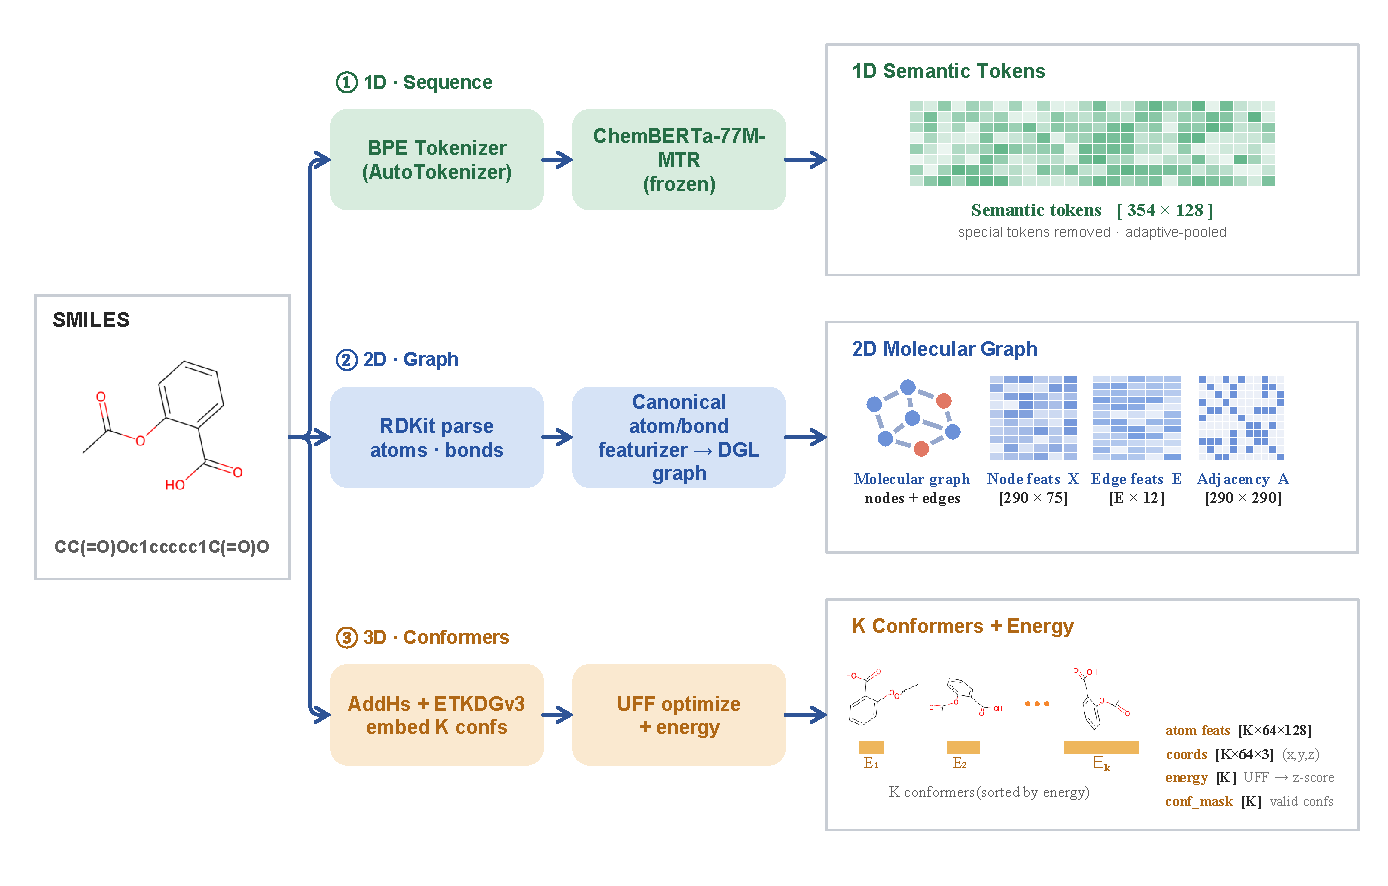
\includegraphics[width=0.98\textwidth,height=0.78\textheight,keepaspectratio]{figures/drug_preprocess.pdf}
\caption{High-resolution version of main-text Figure 1: drug data preprocessing. Starting from a SMILES string, TAMR-DTI constructs a ChemBERTa semantic-token matrix, an RDKit/DGL molecular graph, and a set of energy-ranked 3D conformers with atom features, coordinates, energies, and conformer-validity indicators.}
\label{fig:si_drug_preprocess}
\end{figure}
\clearpage

\begin{figure}[p]
\centering
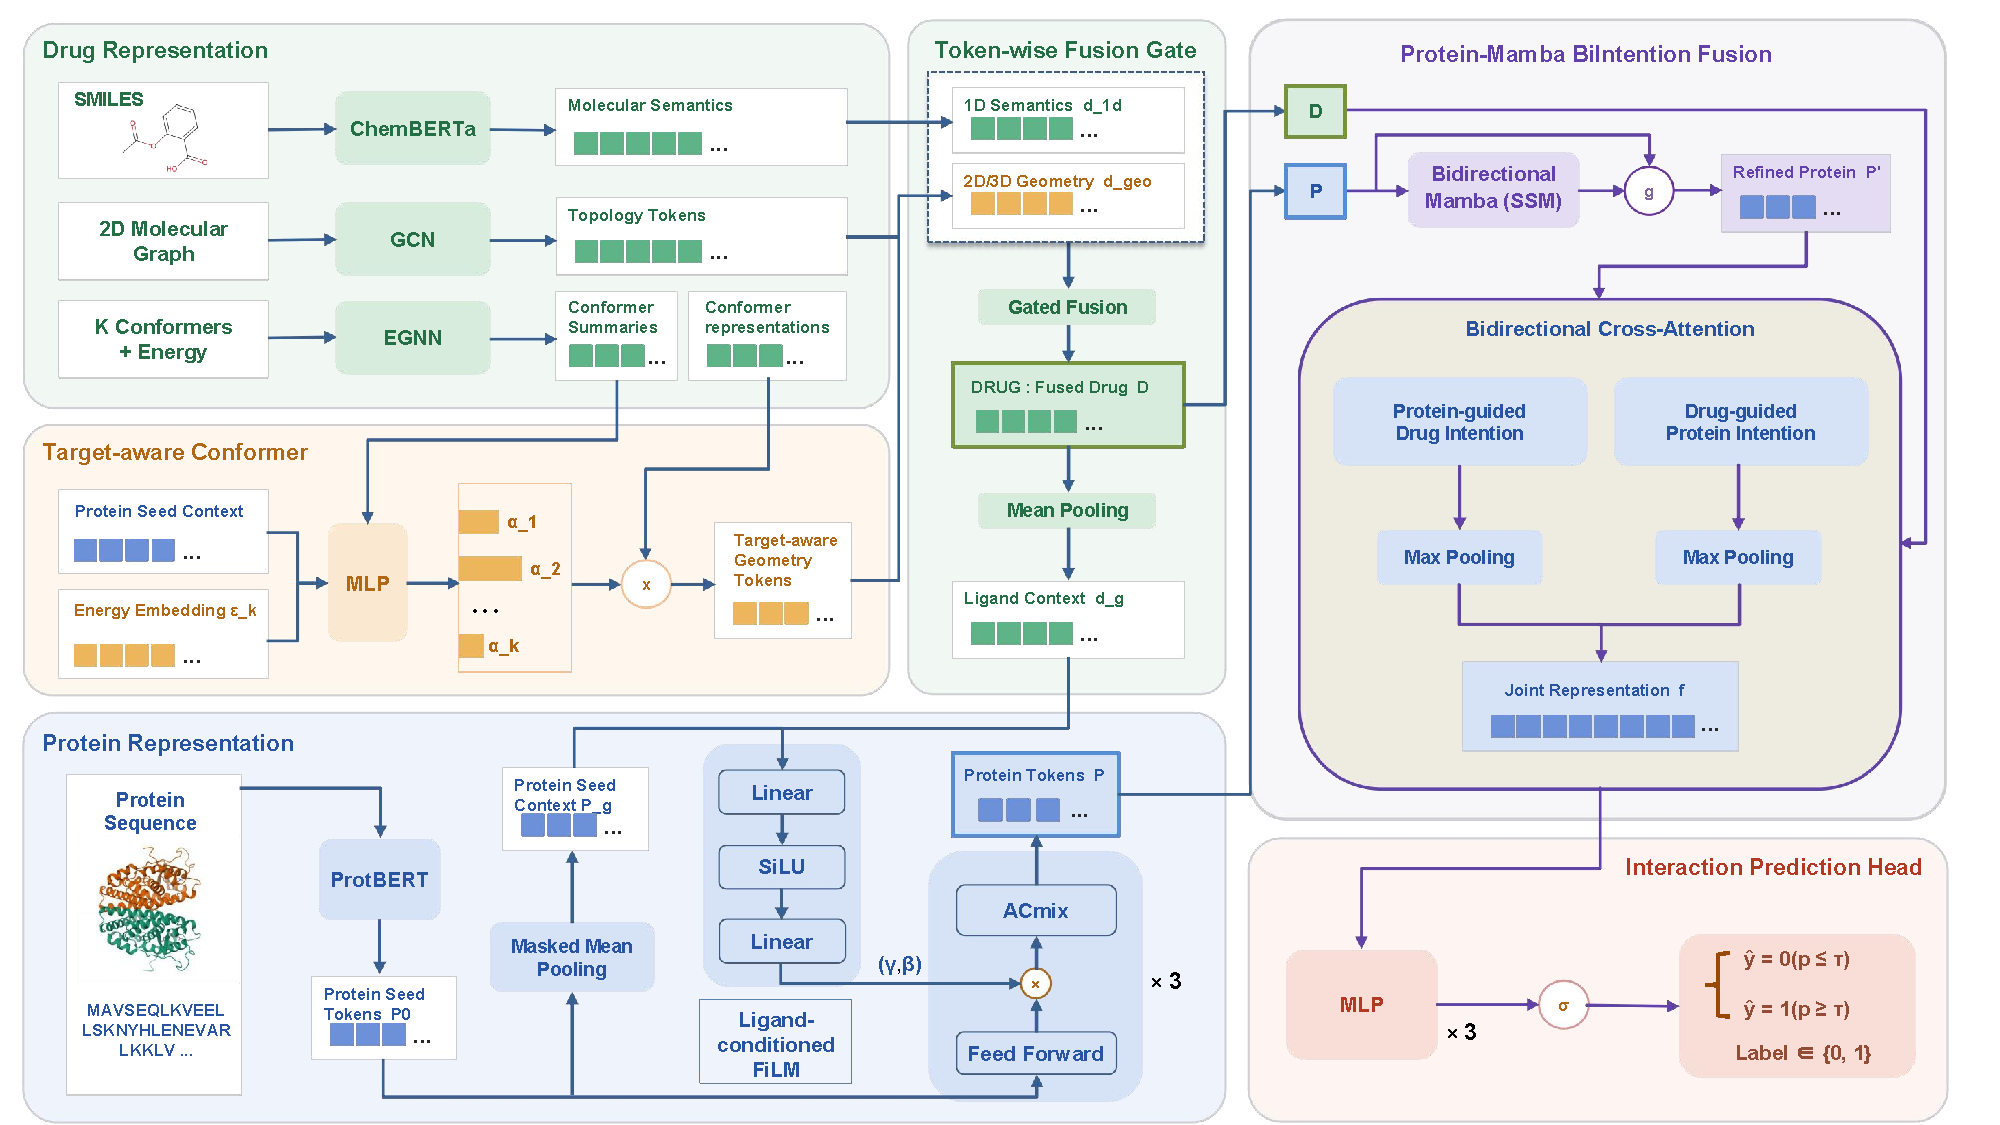
\includegraphics[width=0.98\textwidth,height=0.78\textheight,keepaspectratio]{figures/tamr_dti_architecture.pdf}
\caption{High-resolution version of main-text Figure 2: TAMR-DTI representation framework. The artwork shows the drug representation streams, ligand-conditioned protein representation module, protein-side refinement block, and BiIntention interaction head.}
\label{fig:si_tamr_dti_architecture}
\end{figure}
\clearpage

\begin{figure}[p]
\centering
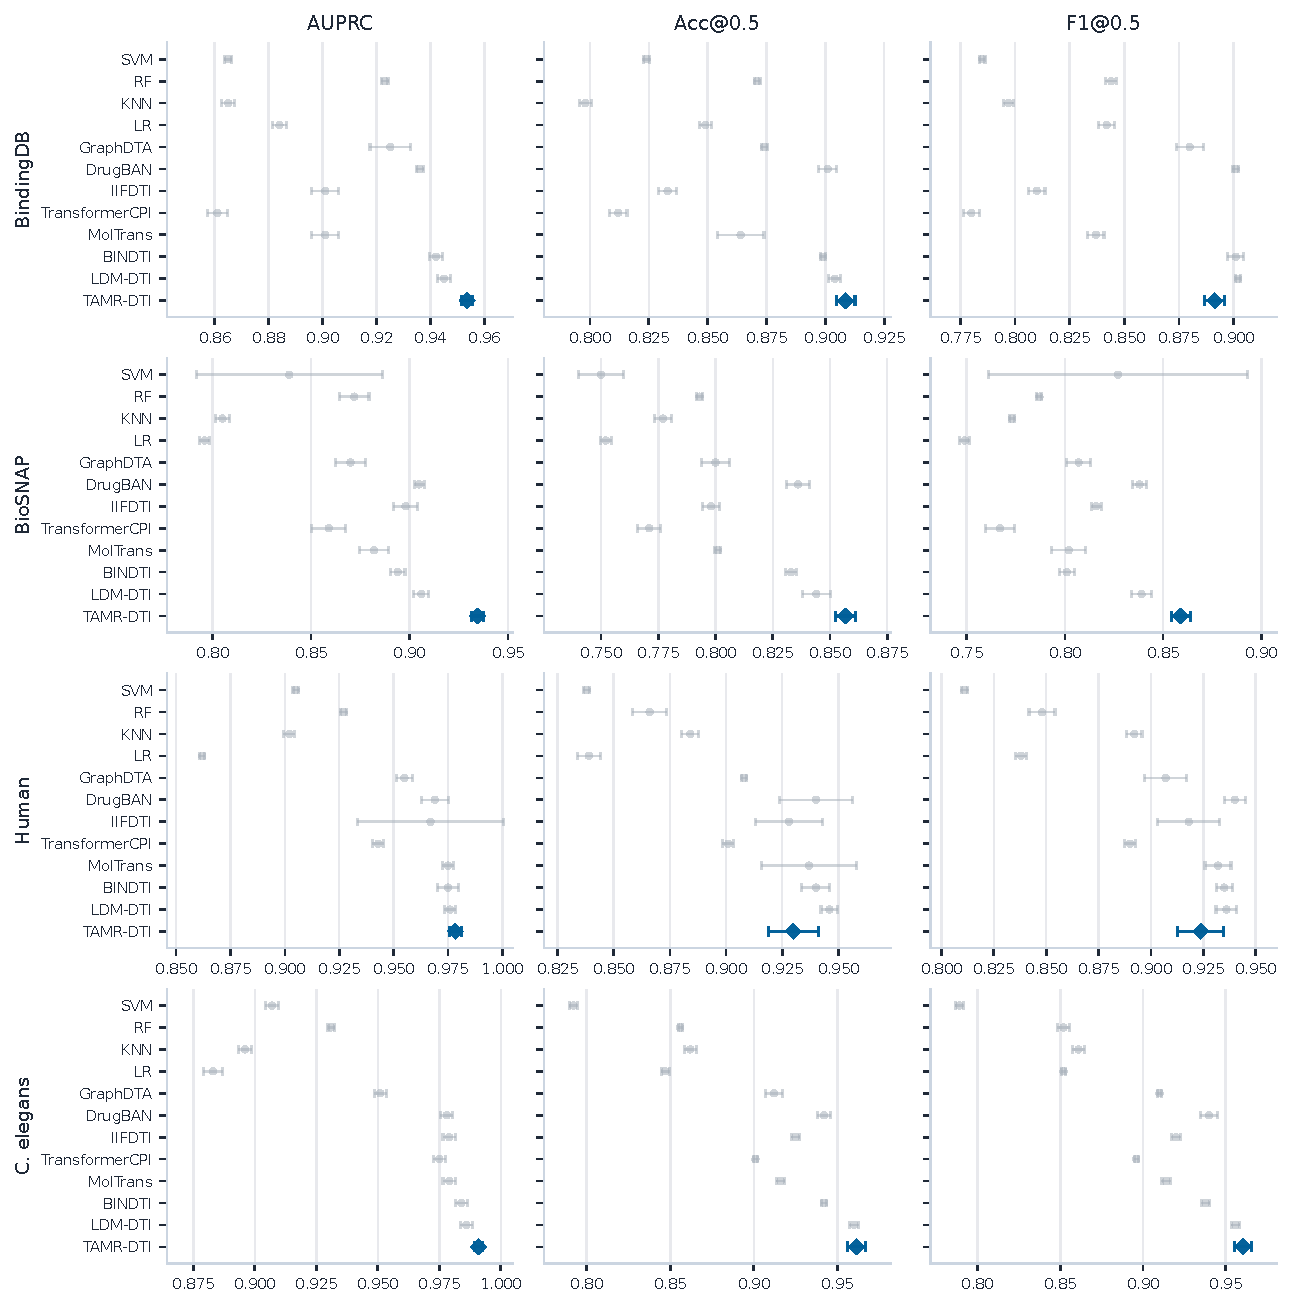
\includegraphics[width=0.98\textwidth,height=0.78\textheight,keepaspectratio]{figures/all_method_ci_comparison.pdf}
\caption{High-resolution version of the main-text all-method comparison figure. The plot shows metric values and uncertainty intervals for AUROC, AUPRC, Acc@0.5, and F1@0.5 across the four benchmark datasets.}
\label{fig:si_all_method_ci_comparison}
\end{figure}
\clearpage

\begin{figure}[p]
\centering
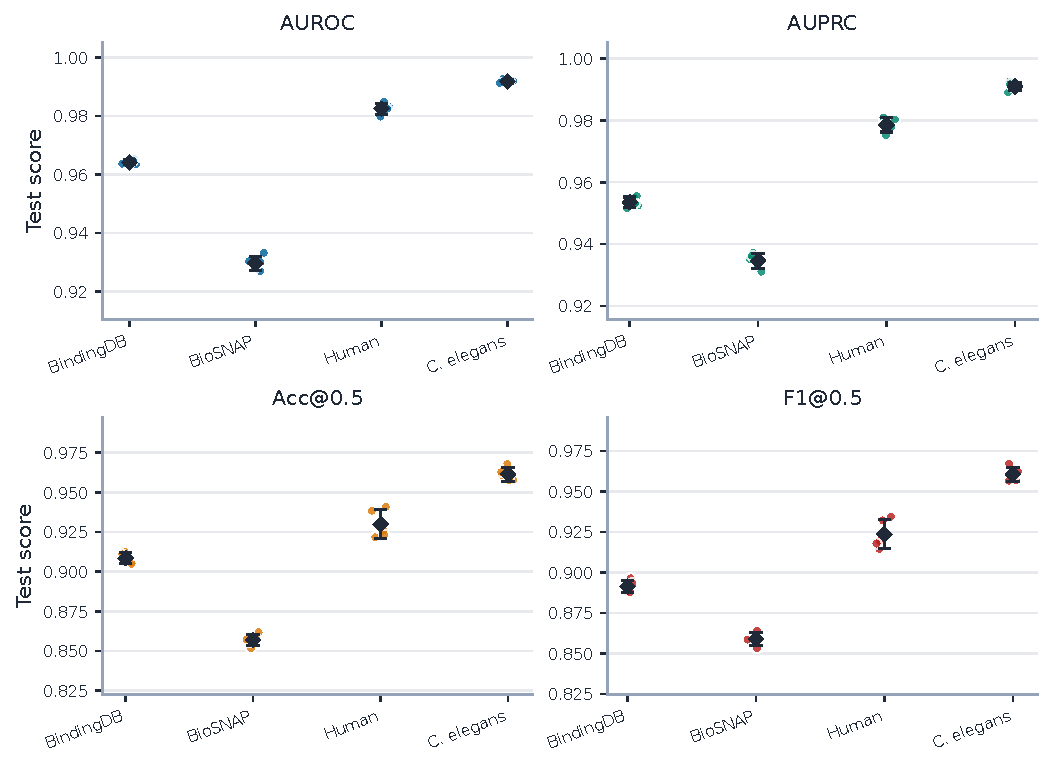
\includegraphics[width=0.98\textwidth,height=0.78\textheight,keepaspectratio]{figures/main_seed_stability.pdf}
\caption{High-resolution version of the main-text seed-stability figure. Each point represents one fixed-seed run and the intervals summarize the repeated-run variation under the stated evaluation protocol.}
\label{fig:si_main_seed_stability}
\end{figure}
\clearpage

\begin{figure}[p]
\centering
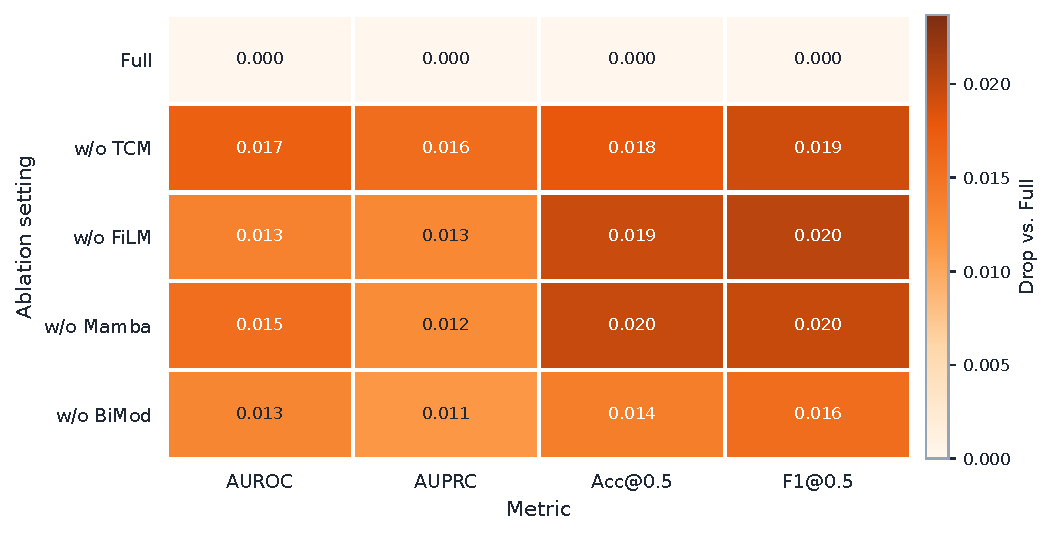
\includegraphics[width=0.98\textwidth,height=0.78\textheight,keepaspectratio]{figures/ablation_biosnap_seed42_drop.pdf}
\caption{High-resolution version of the main-text BioSNAP ablation-drop figure. Each cell reports the relative test-score decrease caused by removing one module under the same seed, split, checkpoint selection rule, and fixed threshold; the complete model is the zero-drop reference.}
\label{fig:si_biosnap_ablation_drop}
\end{figure}
\clearpage

\begin{figure}[p]
\centering
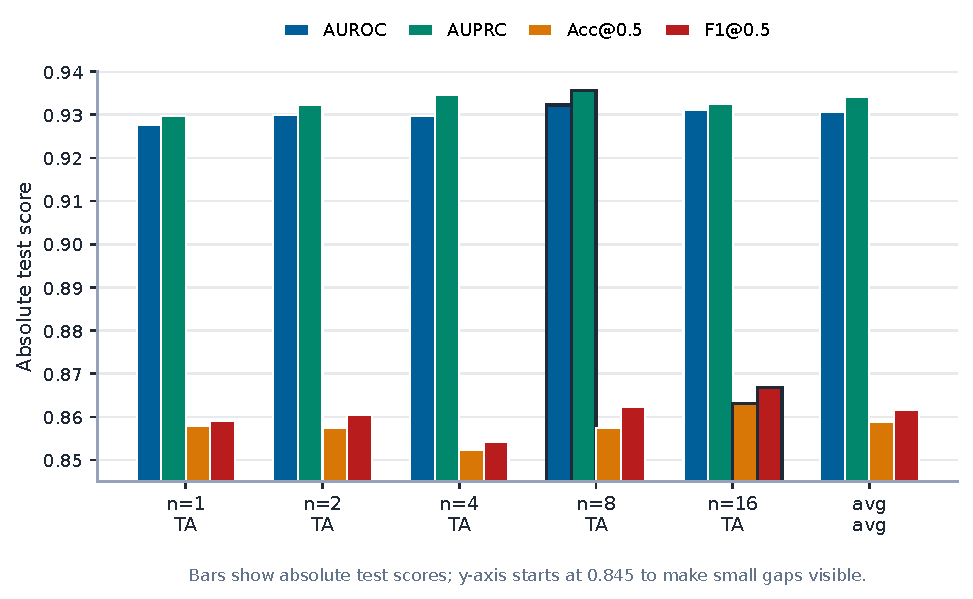
\includegraphics[width=0.98\textwidth,height=0.78\textheight,keepaspectratio]{figures/conformer_biosnap_seed42_comparison.pdf}
\caption{High-resolution version of the main-text conformer-count comparison figure. The plot compares effective conformer counts and uniform versus target-aware aggregation on BioSNAP under the single-seed diagnostic protocol.}
\label{fig:si_biosnap_conformer_comparison}
\end{figure}
\clearpage

\begin{figure}[p]
\centering
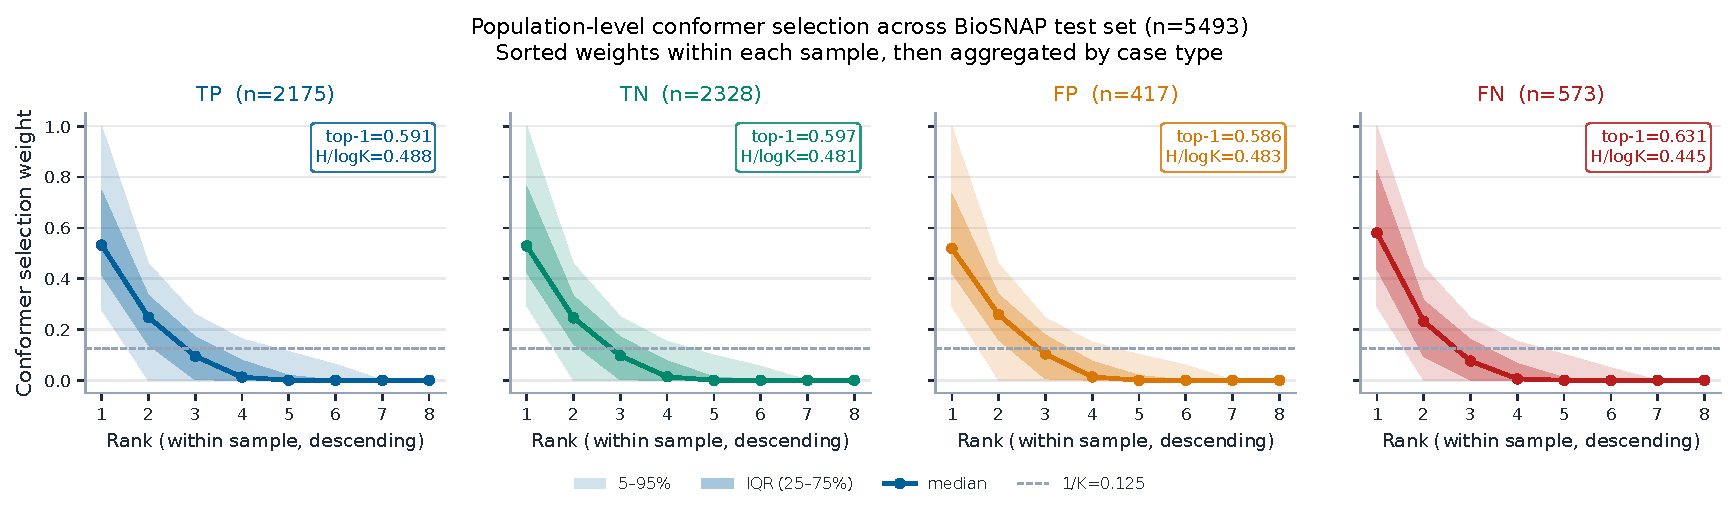
\includegraphics[width=0.98\textwidth,height=0.78\textheight,keepaspectratio]{figures/interpretability_conformer_weights.pdf}
\caption{High-resolution version of the main-text interpretability figure. For each BioSNAP test pair, the eight conformer weights are sorted within the sample and summarized by prediction group; solid curves are medians, dark bands are interquartile ranges, and light bands are the 5--95\% ranges.}
\label{fig:si_interpretability_conformer_weights}
\end{figure}
\clearpage

\FloatBarrier
